\chapter{Проектирование составляющих}

\section{Проектирование МШУ1}

Создадим схему усилителя.
Чтобы добавить усилитель как внешний компонент, добавим на схему блок, позволяющий задать компонент по S-параметрам.

\begin{figure}[!ht]
    \centering
    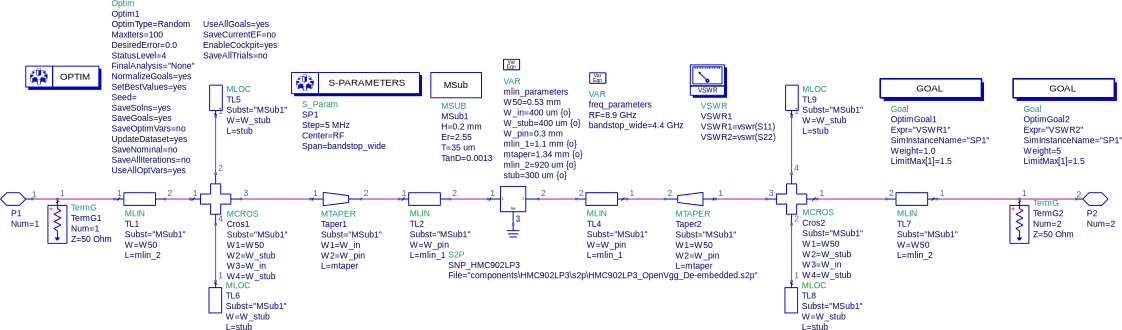
\includegraphics[width=\textwidth]{amplifier_1_schematic.pdf}
    \caption{Внутренняя схема МШУ1}%
    \label{fig:amplifier_1_schematic}
\end{figure}

Проведя моделирование, обнаружим, что КСВН в рабочей полосе не очень хороший.
Для исправления этого поставим крестообразные цепи согласования и параметризуя их параметры, проведём оптимизацию, установив $VSWR1 < 1.5$ и $VSWR2 < 1.5$ как целевые значения оптимизации.

Итоговый вид схемы можно увидеть на Рис.~\ref{fig:amplifier_1_schematic}, а результаты моделирования на Рис.~\ref{fig:amplifier_1_data}.
Результат приемлемый.

\begin{figure}[!ht]
    \centering
    \begin{subfigure}[b]{0.35\textwidth}
        \centering
        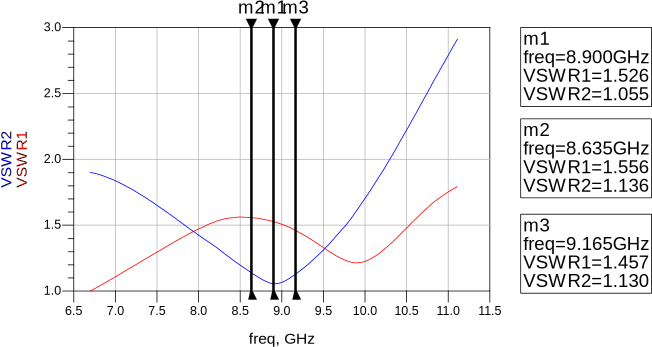
\includegraphics[width=\textwidth]{amplifier_1_data_VSWR.pdf}
        \caption{}%
        \label{fig:amplifier_1_data_VSWR}
    \end{subfigure}
    \hfill
    \begin{subfigure}[b]{0.35\textwidth}
        \centering
        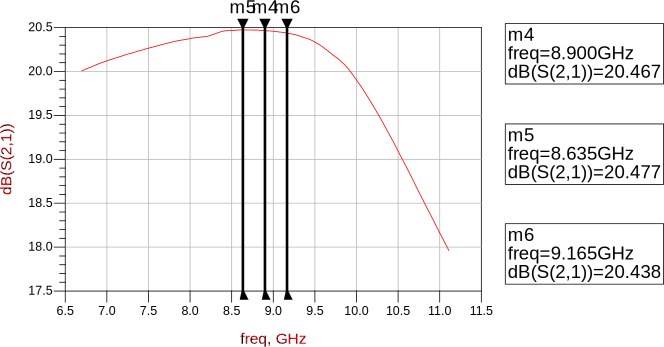
\includegraphics[width=\textwidth]{amplifier_1_data_response.pdf}
        \caption{}%
        \label{fig:amplifier_1_data_response}
    \end{subfigure}
    \caption{%
        Частотные характеристики проектируемого усилителя:
        (а) КСВН;
        (б) АЧХ
    }%
    \label{fig:amplifier_1_data}
\end{figure}

\section{Проектирование фильтра}

Создадим схему фильтра.
Чтобы добавить фильтр как внешний компонент, добавим на схему блок, позволяющий задать компонент по S-параметрам.
Проектирование фильтра велось в среде Keysight Genesys.

\begin{figure}[!ht]
    \centering
    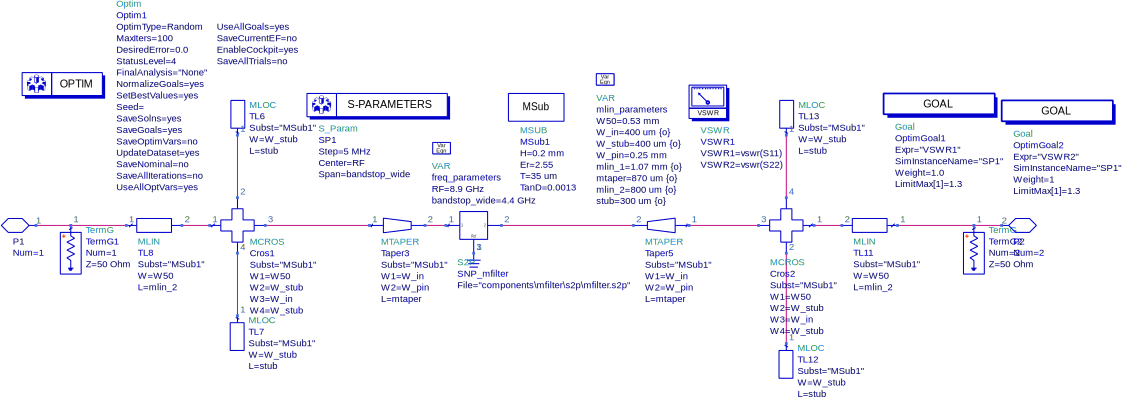
\includegraphics[width=\textwidth]{filter_schematic.pdf}
    \caption{Внутренняя схема фильтра}%
    \label{fig:filter_schematic}
\end{figure}

Проведя моделирование, обнаружим, что КСВН в рабочей полосе не очень хороший.
Для исправления этого поставим крестообразные цепи согласования и параметризуя их параметры, проведём оптимизацию, установив $VSWR1 < 1.3$ и $VSWR2 < 1.3$ как целевые значения оптимизации.

Итоговый вид схемы можно увидеть на Рис.~\ref{fig:filter_schematic}, а результаты моделирования на Рис.~\ref{fig:filter_data_response}.
Результат приемлемый.

\begin{figure}[!ht]
    \centering
    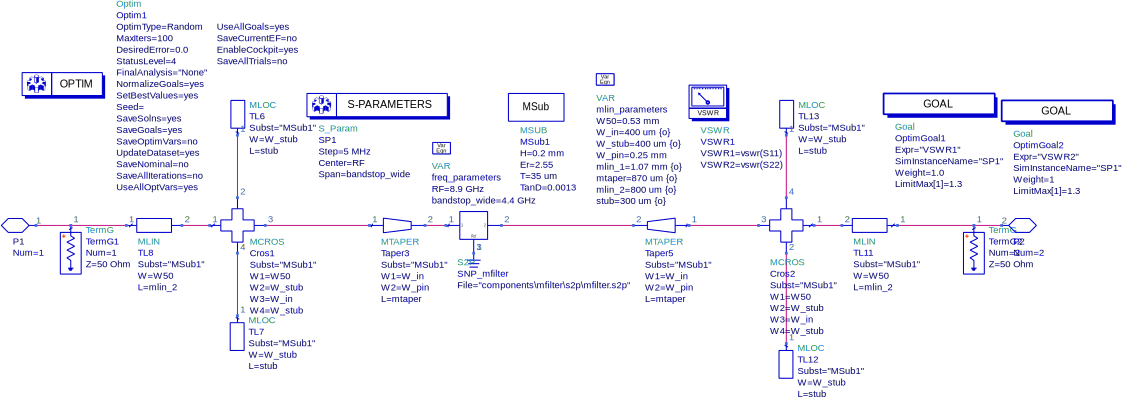
\includegraphics[width=\textwidth]{filter_data_response.pdf}
    \caption{АЧХ проектируемого фильтра}%
    \label{fig:filter_data_response}
\end{figure}

\section{Проектирование фазовращателя}

Создадим схему фазовращателя.
Чтобы добавить фазовращатель как внешний компонент, добавим на схему блок, позволяющий задать компонент по S-параметрам.

\begin{figure}[!ht]
    \centering
    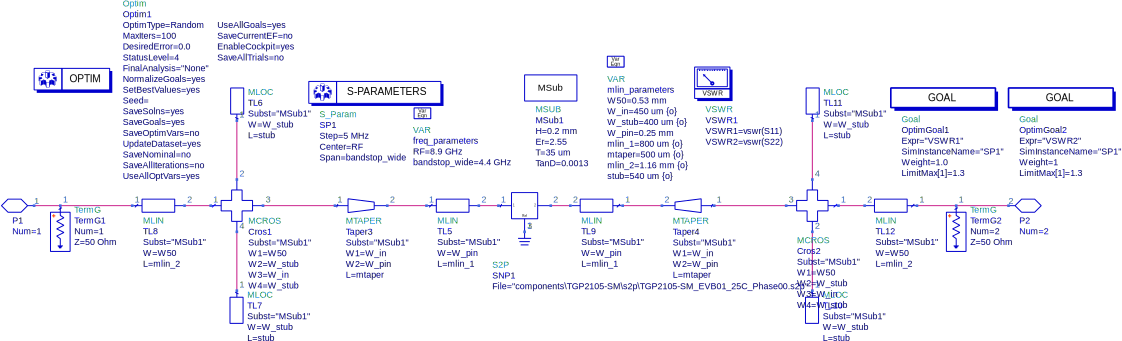
\includegraphics[width=\textwidth]{phase_shifter_schematic.pdf}
    \caption{Внутренняя схема фазовращателя}%
    \label{fig:phase_shifter_schematic}
\end{figure}

Проведя моделирование, обнаружим, что КСВН в рабочей полосе не очень хороший.
Для исправления этого поставим крестообразные цепи согласования и параметризуя их параметры, проведём оптимизацию, установив $VSWR1 < 1.3$ и $VSWR2 < 1.3$ как целевые значения оптимизации.

Итоговый вид схемы можно увидеть на Рис.~\ref{fig:phase_shifter_schematic}, а результаты моделирования на Рис.~\ref{fig:phase_shifter_data_VWSR}.
Результат приемлемый.

\begin{figure}[!ht]
    \centering
    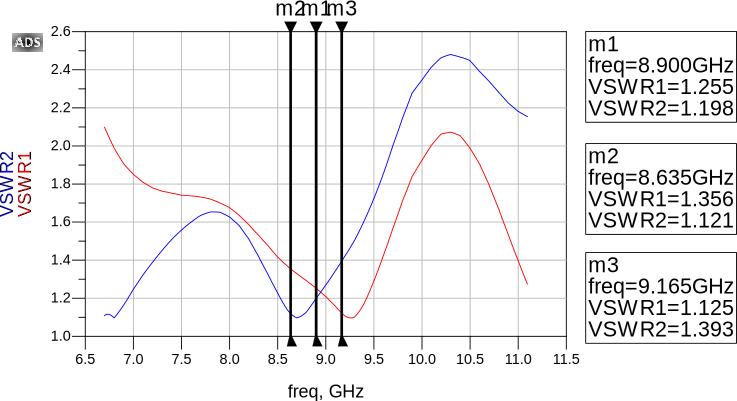
\includegraphics[width=0.8\textwidth]{phase_shifter_data_VWSR.pdf}
    \caption{Зависимость КСВН фазовращателя от частоты}%
    \label{fig:phase_shifter_data_VWSR}
\end{figure}

\section{Проектирование МШУ2}

Создадим схему усилителя.
Чтобы добавить усилитель как внешний компонент, добавим на схему блок, позволяющий задать компонент по S-параметрам.

\begin{figure}[!ht]
    \centering
    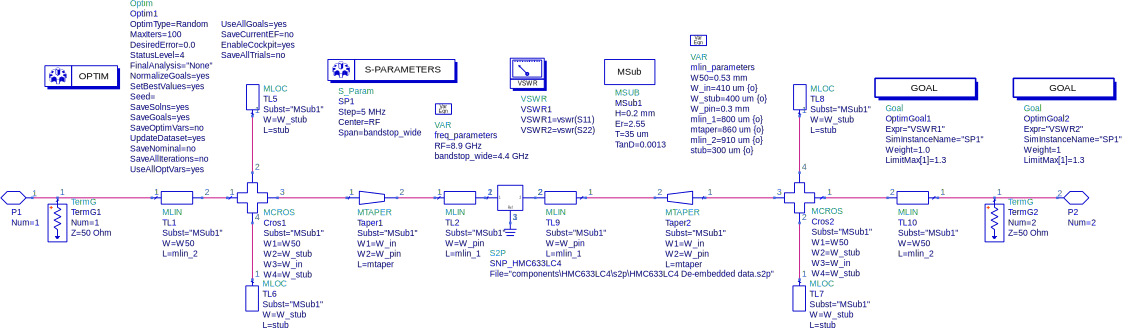
\includegraphics[width=\textwidth]{amplifier_2_schematic.pdf}
    \caption{Внутренняя схема МШУ2}%
    \label{fig:amplifier_2_schematic}
\end{figure}

Проведя моделирование, обнаружим, что КСВН в рабочей полосе не очень хороший.
Для исправления этого поставим крестообразные цепи согласования и параметризуя их параметры, проведём оптимизацию, установив $VSWR1 < 1.5$ и $VSWR2 < 1.5$ как целевые значения оптимизации.

Итоговый вид схемы можно увидеть на Рис.~\ref{fig:amplifier_2_schematic}, а результаты моделирования на Рис.~\ref{fig:amplifier_2_data}.
Результат приемлемый.

\begin{figure}[!ht]
    \centering
    \begin{subfigure}[b]{0.45\textwidth}
        \centering
        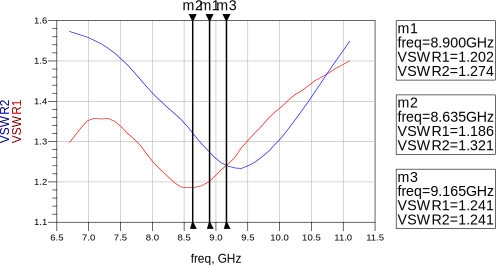
\includegraphics[width=\textwidth]{amplifier_2_data_VSWR.pdf}
        \caption{}%
        \label{fig:amplifier_2_data_VSWR}
    \end{subfigure}
    \hfill
    \begin{subfigure}[b]{0.45\textwidth}
        \centering
        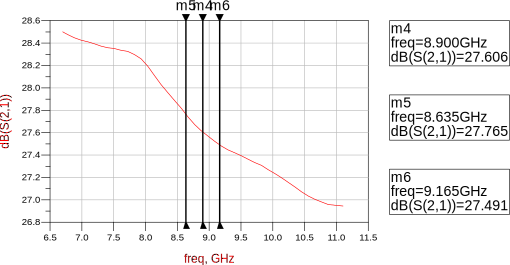
\includegraphics[width=\textwidth]{amplifier_2_data_response.pdf}
        \caption{}%
        \label{fig:amplifier_2_data_response}
    \end{subfigure}
    \caption{%
        Частотные характеристики проектируемого усилителя:
        (а) КСВН;
        (б) АЧХ
    }%
    \label{fig:amplifier_2_data}
\end{figure}

